\subsection{Mô hình dịch Việt - Lào}

Tầng thứ ba của hệ thống nhận câu tiếng Việt đã được chuẩn hóa từ mô-đun trước và dịch
sang tiếng Lào. Nếu mô-đun ghép câu giúp đầu ra trở nên tự nhiên trong nội ngữ, thì mô
đun này mở rộng hệ thống sang giao tiếp liên ngôn ngữ. Trong bối cảnh của đồ án, đây là
khâu biến một pipeline nhận diện ký hiệu thành một pipeline truyền đạt thông tin cho người
dùng ở ngôn ngữ khác.

Tài liệu mô tả ban đầu trong \texttt{vilo.pdf} trình bày các khái niệm nền như
\textit{Sequence-to-Sequence}, \textit{Attention}, \textit{Transformer} và
\textit{Embedding}. Đối chiếu với mã nguồn thực tế, project hiện tại hiện thực hóa các ý
tưởng đó bằng mô hình NLLB-200 Distilled 600M kết hợp adapter LoRA, thay vì dùng một
kiến trúc Seq2Seq tự xây từ đầu.

\begin{figure}[H]
\centering
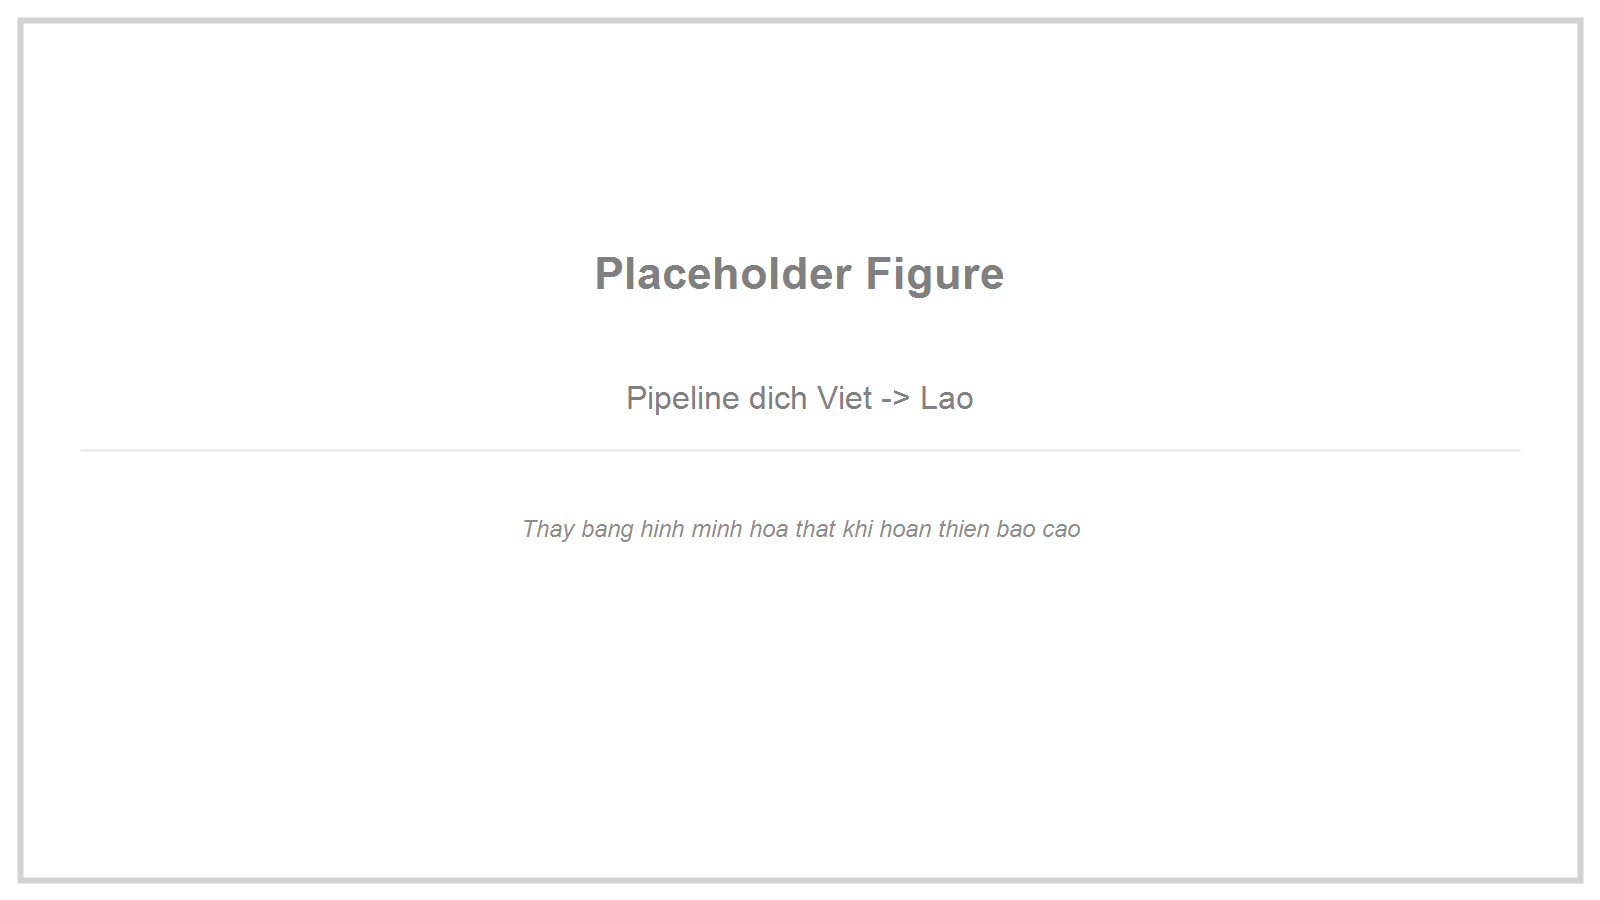
\includegraphics[width=0.88\textwidth]{figures/translation/vi_lao_mt_pipeline.png}
\caption{Vị trí của mô-đun dịch Việt - Lào trong pipeline tổng thể}
\label{fig:vi-lao-pipeline}
\end{figure}

\subsubsection{Bài toán dịch máy trong phạm vi đề tài}

Đầu vào của mô-đun là câu tiếng Việt đã qua tầng sửa ngữ pháp, ví dụ
\textit{Tôi muốn uống nước.} hoặc \textit{Tôi cần giúp đỡ.} Đầu ra mong muốn là câu
tiếng Lào tương đương về nghĩa, đủ tự nhiên để có thể hiển thị hoặc kết hợp với các tầng
hỗ trợ giao tiếp khác như text-to-speech.

Xét về mặt học máy, đây là bài toán dịch máy \textit{text-to-text}. Mô hình không chỉ cần
dịch đúng từ vựng, mà còn phải bảo toàn vai nghĩa, trật tự thông tin và cách dùng từ theo
đúng ngữ cảnh. Điều này đặc biệt quan trọng khi hệ thống phục vụ các tình huống giao
tiếp hỗ trợ, nơi một sai lệch nhỏ về nghĩa có thể làm thay đổi ý định của người dùng.

\subsubsection{Lý do chọn NLLB-200 Distilled 600M}

NLLB (\textit{No Language Left Behind}) là họ mô hình dịch máy đa ngôn ngữ do Meta
phát triển với mục tiêu hỗ trợ các ngôn ngữ tài nguyên thấp. Theo NLLB Team, công trình
này tập trung thu hẹp khoảng cách hiệu năng giữa ngôn ngữ giàu và nghèo tài nguyên, đồng
thời đánh giá trên hơn 40.000 hướng dịch và hướng tới mốc 200 ngôn ngữ. Với một
đề tài có cặp ngôn ngữ Việt - Lào, đây là một lựa chọn hợp lý vì tiếng Lào là ngôn ngữ ít
tài nguyên hơn nhiều so với các cặp dịch phổ biến như Anh - Pháp hoặc Anh - Đức.

Project sử dụng biến thể \texttt{nllb-200-distilled-600M}. So với các bản lớn hơn, bản
\textit{distilled 600M} cho phép:
\begin{itemize}
    \item giảm yêu cầu phần cứng, phù hợp hơn với môi trường triển khai học thuật;
    \item giữ được lợi thế của tiền huấn luyện đa ngôn ngữ;
    \item thuận tiện hơn khi tinh chỉnh bằng adapter thay vì full fine-tuning.
\end{itemize}

Vì đầu vào của mô-đun đã là câu tiếng Việt sạch ngữ pháp, NLLB đóng vai trò như một
khối dịch máy chuyên dụng nằm ở cuối pipeline, tận dụng kiến thức đa ngôn ngữ có sẵn
thay vì phải xây toàn bộ mô hình dịch mới từ đầu.

\subsubsection{Chiến lược tinh chỉnh bằng LoRA}

LoRA (\textit{Low-Rank Adaptation}) là kỹ thuật tinh chỉnh tham số hiệu quả, trong đó mô
hình gốc được giữ cố định và chỉ thêm các ma trận hạng thấp có khả năng học vào một số
lớp của Transformer. Theo Hu và cộng sự, cách làm này giúp giảm mạnh số tham số cần
cập nhật nhưng vẫn duy trì chất lượng tốt trên các tác vụ downstream.

Tệp \texttt{adapter\_config.json} trong project cho thấy adapter hiện tại có cấu hình:
\begin{itemize}
    \item \texttt{r = 16};
    \item \texttt{lora\_alpha = 32};
    \item \texttt{lora\_dropout = 0.05};
    \item áp dụng trên các module \texttt{q\_proj}, \texttt{k\_proj},
    \texttt{v\_proj} và \texttt{out\_proj};
    \item kiểu tác vụ: \texttt{SEQ\_2\_SEQ\_LM}.
\end{itemize}

Như vậy, project không huấn luyện lại toàn bộ NLLB mà chỉ học một lớp thích nghi mỏng
trên đỉnh mô hình nền. Đây là lựa chọn rất phù hợp với đồ án sinh viên vì vừa tiết kiệm tài
nguyên, vừa cho phép lưu trữ mô hình dưới dạng adapter nhỏ gọn.

\begin{figure}[H]
\centering
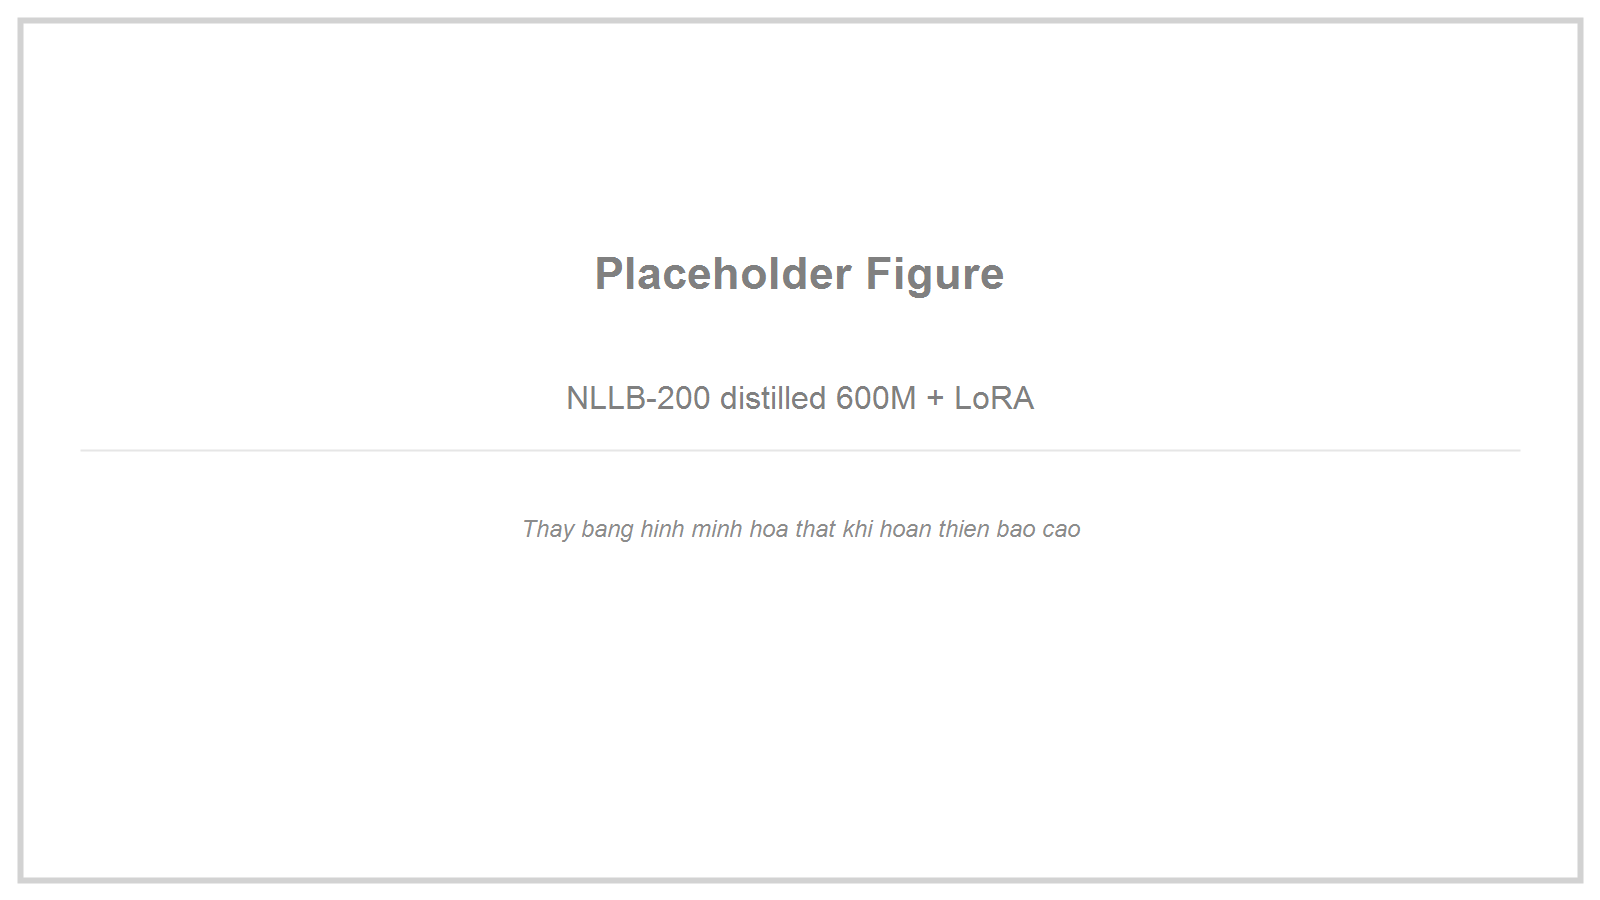
\includegraphics[width=0.84\textwidth]{figures/translation/nllb_lora_architecture.png}
\caption{Kiến trúc NLLB-200 kết hợp adapter LoRA trong mô-đun dịch Việt - Lào}
\label{fig:nllb-lora-architecture}
\end{figure}

\subsubsection{Tokenizer và cơ chế sinh câu đích}

Theo tài liệu chính thức của Hugging Face cho NLLB, tokenizer của họ mô hình này sử
dụng mã ngôn ngữ nguồn và ngôn ngữ đích như các \textit{special tokens}. Trong project,
quá trình suy luận được cấu hình như sau:
\begin{itemize}
    \item ngôn ngữ nguồn: \texttt{vie\_Latn};
    \item ngôn ngữ đích: \texttt{lao\_Laoo};
    \item ép token bắt đầu của câu đích bằng \texttt{forced\_bos\_token\_id};
    \item \texttt{max\_length = 128};
    \item \texttt{num\_beams = 5}.
\end{itemize}

Thiết kế này rất quan trọng. Nếu không đặt đúng mã ngôn ngữ hoặc không ép token bắt đầu
của tiếng đích, mô hình đa ngôn ngữ có thể sinh sai ngôn ngữ hoặc lẫn giữa nhiều miền dữ
liệu. Việc dùng \texttt{beam search} với 5 nhánh cũng cho phép mô hình ưu tiên những câu
dịch ổn định hơn so với giải mã tham lam đơn giản.

\subsubsection{Ưu điểm và những rủi ro cần lưu ý}

Điểm mạnh của hướng tiếp cận hiện tại là tận dụng được tri thức tiền huấn luyện đa ngôn
ngữ của NLLB, đồng thời dùng LoRA để hạ chi phí huấn luyện và lưu trữ. Điều này khiến
module dịch phù hợp với bối cảnh nghiên cứu ứng dụng, nơi khối lượng phần cứng thường
không đủ để full fine-tune các mô hình dịch cỡ lớn.

Tuy nhiên, mô-đun vẫn tồn tại một số rủi ro kỹ thuật:
\begin{itemize}
    \item chất lượng dịch phụ thuộc trực tiếp vào câu tiếng Việt đầu vào; nếu mô-đun ghép
    câu phía trước diễn đạt sai ý, mô-đun dịch sẽ khuếch đại lỗi đó;
    \item dữ liệu song ngữ hiện có khá dị miền, bao gồm hội thoại, câu kể, tên riêng và các
    câu mô tả dài, nên dễ phát sinh lỗi với thực thể riêng hoặc câu khẩu ngữ;
    \item một số mẫu dữ liệu quan sát được cho thấy còn hiện tượng nhiễu chính tả, viết hoa
    hoặc phiên âm tên riêng, có thể làm giảm tính ổn định của đầu ra.
\end{itemize}

Vì vậy, khi đánh giá mô-đun này, không nên chỉ nhìn vào một ví dụ dịch thành công, mà
cần đánh giá đồng thời bằng các metric dịch máy chuẩn và các ví dụ định tính nhiều miền.

